\section{Evaluation}
\label{sec:eval}

The target of this section is two fold presented in the following two case studies.
First, we demonstrate the severity of conducting \drop attack on the closest peers to the source.
Second, we evaluate the proposed detection mechanism's performance, accuracy and the overhead induced on the system due to the messages exchanged by the different detection steps.
First we describe the simulation framework and the parameters for different simulation configurations. Afterwards the metrics used in both case studies are provided.
Finally, we detail the simulation results and the interpretation in both case studies.

\subsection{Simulation Framework and Parameters}
Our simulation framework is based on OSSim \cite{nguyen2013ossim}. 
OSSim provides a packet level simulator for DONet \cite{zhang2005coolstreaming}, a pull-based online video streaming overlay, which we use in our case studies.
We use the network topology generator GT-ITM \cite{GT} with 1000 peers connected to 400 edge router.

To simulate for the worst case scenarios, we assume malicious peers never leave the overlay once they join.
However, to emulate real life measurements \cite{distribution}, benign peers joining is based on Pareto distribution, while their leaving times is estimated using Lognormal distributions.
Benign peers can rejoin the overlay in a uniform distribution around 10s.

As our proposed attack aims at attacking the overlay once the source starts to send video chunks, we focus on showing both the attack's impact along with the detection mechanism's performance on simulation time of 500s.
The results are calculated over 10 runs for each simulation configuration.

The parameters used in both case studies are provided in Table \ref{tab:parameters}.

\begin{table}[ht]
\center
\caption{Acronyms}
\begin{tabular}{|c|c||c|c|}
\hline

\bf{Var.} & \bf{Desc.}  & \bf{Var.} & \bf{Desc.} \\\hline\hline

mal. headnodes $\eta x$ & $\{5,8,10\}$ & chunk size & 2500B \\\hline
sat. threshold $\satThres$ & $\{0.5,0.7,0.95\}$ & $\treply$ & 10s\\\hline
mal. neighbors $MN$  & $\{0,15,24,49,100\}$ & stream Rate & 400kbps\\\hline
min. responses $\minP$ &  $\{3,4\}$ & buffer size & 30s  \\\hline
det. allowed $\minDR$ & 10 & list size $LS$ & $\{8,10\}$\\\hline
  
\end{tabular}
\label{tab:parameters}
\end{table}

\subsection{Metrics}

Here we define the metrics used throughout the evaluation.
\subsubsection*{Satisfaction $\sat$} which represents the average peer satisfaction level through the whole simulation interval.
\subsubsection*{Avg. Loss} that indicates the avg chunk loss per peer.
\subsubsection*{Detection Overhead $DO$} used to evaluate the detection overhead induced on the system, i.e., the ratio of messages exchanged during due to the detection mechanism over all signaling messages in the system.
\subsubsection*{Malicious Ratio per Neighbor List $MRNL$} which measures the ratio of malicious peers over all peers in benign peers neighbor list.

\subsection{Case 1: \drop Severity}

In this case study, we evaluate the impact of \drop attack on two different network scenarios:  (1) DONet, and (2) DONet+SWAP \cite{nguyen2016swap}, in order to assess the attack's severity when a replacement mechanism for peers is operating.
Note that the attacker's budget is independent from the overlay's size, in fact, the attacker's budget is dependent on the neighbor list size $LS$.
The reason is that as malicious peers target is to occupy the closest peers to the source, the remaining size of the overlay is not a factor on the impact of the \drop attack.
As the neighbor list size is $LS=10,8$ , respectively, we choose the following combinations for the attackers budget $x={\{\eta x, MN\}}$: $\{10=\{10,0\}\}, \{20=\{5,15\}\}, 56=\{7,49\}\}, 32=\{8,24\}\}$.
For example, $MN=49$ implies that 7 malicious peers are connected to each of the 10 headnodes.

\subsubsection{DONet}
In Figure~\ref{subfig:avg-loss-donet}, the average chunk loss is presented. 
Obviously, the average loss is 100\% when $\eta x= LS =10$, which means that all the source's $LS$ is occupied with malicious headnodes, i.e., no chunks are passed to the overlay.
Accordingly, the average peer satisfaction in such case is inevitably 0\%. 

For other cases, where $\eta x < 10$, at $x=\{7, 49\}$ the average loss when the stream starts reaches up to ~82\%, at $x=\{5, 3\}$, where the chunks loss is ~54\%, As shown in Figure~\ref{subfig:avg-loss-donet}.
For the case of having high $\eta x$ and relatively low $MN$ ($x=\{8, 3\}$), the chunk loss is ~73\%.

% it is noticed that the impact of the attack is significantly successful in dropping the chunk success delivery ratio up to ~82\% once the source starts to send video chunks.
It is inferred that depending on the value of $\eta x, MN$, benign peers starve for a longer period of time till they are served as benign peers closer to the source are overloaded with requests that they can not utterly serve. 
Eventually, the loss ratio decreases after a fraction of benign (headnodes and non-headnodes) peers are able to serve the rest of the overlay.
Figure~\ref{subfig:satisfaction-donet} illustrates the average peer satisfaction level $\sat$ is assessed.
As a consequence of experiencing high chunk loss, higher values of $\eta x, MN$ results in lower peer satisfaction over time, where benign peers at $x=\{5, 3\}$ restore their $\sat$ at ~340s, earlier than at $x=\{7, 7\}$ and $x=\{8, 3\}$.

\begin{figure}[t!]
\centering

%   \mbox{\subfloat[Avg. loss]{\label{subfig:avg-loss-donet}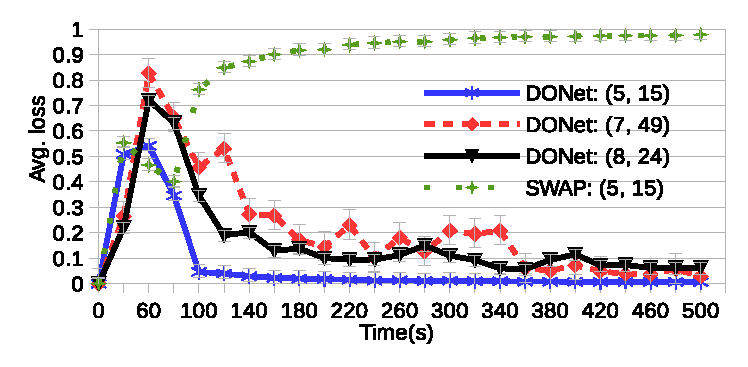
\includegraphics[width=8.4cm,height=3.5cm]{./Figures/avg-loss-donet.eps}}}
%  
%   \mbox{\subfloat[Avg. peer satisfaction]{\label{subfig:satisfaction-donet}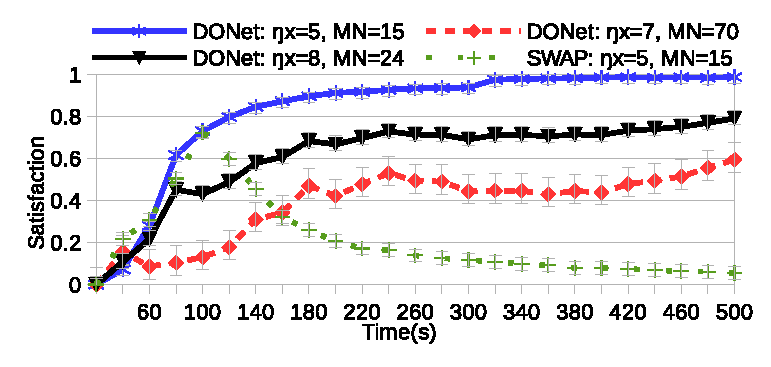
\includegraphics[width=8.4cm,height=3.5cm]{./Figures/satisfaction-donet.eps}}}
  \mbox{\subfloat[Avg. loss]{\label{subfig:avg-loss-donet}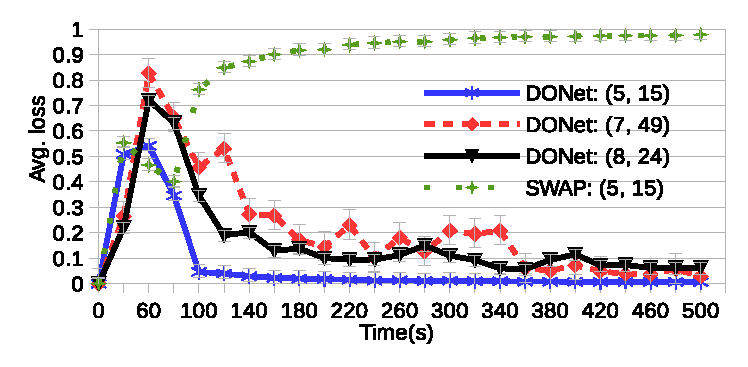
\includegraphics[width=3.7cm,height=2.5cm]{./Figures/avg-loss-donet.eps}} \subfloat[Avg. peer satisfaction]{\label{subfig:satisfaction-donet}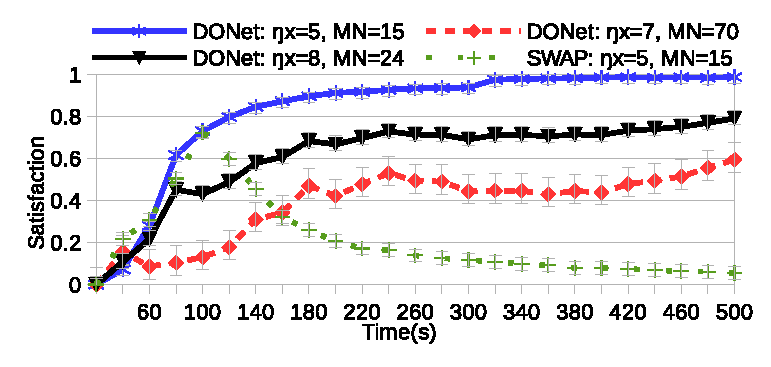
\includegraphics[width=3.7cm,height=2.5cm]{./Figures/satisfaction-donet.eps}}} 
  \caption{Attack's Impact on DONet }
  \label{fig:attack-results}
  \end{figure}


\subsubsection{DONet+SWAP}


\subsection{Case 2: Detection Mechanism Performance}

% 
% The results along with a discussion for each of the two aforementioned case studies are detailed next.
% 
% \subsubsection{Impact of $Hx$}
% Given that the maximum number of neighbors that the source or any other peer can have is $\alpha =10$, it's interesting to see the impact of occupying a certain fraction of the source's neighbor list.
% Figure~\ref{fig:DONet} and Figure~\ref{fig:swap} depict the impact of increasing the fraction of malicious headnodes while keeping the number of malicious neighbors to those malicious headnodes constant.
% 
% For DONet, as long as the source's neighbor list size $\alpha$ is not fully saturated with malicious peers, benign peers $b$ eventually get a stable flow of the video chunks, as depicted in Figure~\ref{subfig:Donet-hx2} through Figure~\ref{subfig:Donet-hx8}.
% Nevertheless, due to the time constraints of such overlay, the fraction of lost chunks is remarkably high once the source starts to generate chunks as the average $IL$ ranges between 49\%-80\% at times 50s-150s. 
% This denotes that once the source starts sending video chunks, benign peers are almost unable to receive those chunks for an intolerant period of time, which is commonly unacceptable for P2P streaming applications' users.
% 
% Figure~\ref{subfig:Donet-hx10} shows the impact of fully exploiting the source's neighbor list neighbors by malicious peers, where in this case $\alpha = Hx$.
% In this case, the average $IL$ is almost 100\%, which denotes benign peers being totally unable to receive video chunks as malicious peers fully acquire all chunks from the source.
% 
% For the attack's impact when SWAP is functioning, which is illustrated in Figure~\ref{fig:swap}, the attack's impact is even worse compared to DONet.
% This is due to that malicious headnodes $Hx$ constantly nominate malicious neighbors $MN$ to the source.
% Eventually, the source acquires $\alpha$ malicious peers in its neighbor list, which in turn causes the $IL$ to reach to ~100\%.
% Indeed, higher values of $Hx$ results in earlier total block of video chunks as shown in Figure~\ref{subfig:swap-hx2} through Figure~\ref{subfig:swap-hx10}.
% Next, the impact of having different values of $MN$ is discussed.
% 
% \begin{figure}[t!]
% \centering
% 
%   \mbox{\subfloat[DONet-$Hx=2$]{\label{subfig:Donet-hx2}\includegraphics[width=7cm,height=4cm]{./Figures/donet-hx2.eps}}}
%   \mbox{\subfloat[DONet-$Hx=5$]{\label{subfig:Donet-hx5}\includegraphics[width=7cm,height=4cm]{./Figures/donet-hx5.eps}}}
%   \mbox{\subfloat[DONet-$Hx=8$]{\label{subfig:Donet-hx8}\includegraphics[width=7cm,height=4cm]{./Figures/donet-hx8.eps}}}
%   \mbox{\subfloat[DONet-$Hx=10$]{\label{subfig:Donet-hx10}\includegraphics[width=7cm,height=4cm]{./Figures/donet-hx10.eps}}}
%    
%   \caption{DONet performance}
% 
%   \label{fig:DONet}
%   \end{figure}
%   
% \begin{figure}[t!]
% \centering
% 
%   \mbox{\subfloat[SWAP-$Hx=2$]{\label{subfig:swap-hx2}\includegraphics[width=7cm,height=4cm]{./Figures/swap-hx2.eps}}}
%   \mbox{\subfloat[SWAP-$Hx=5$]{\label{subfig:swap-hx5}\includegraphics[width=7cm,height=4cm]{./Figures/swap-hx5.eps}}}
%   \mbox{\subfloat[SWAP-$Hx=8$]{\label{subfig:swap-hx8}\includegraphics[width=7cm,height=4cm]{./Figures/swap-hx8-nei5-hops1.eps}}}
%   \mbox{\subfloat[SWAP-$Hx=10$]{\label{subfig:swap-hx10}\includegraphics[width=7cm,height=4cm]{./Figures/swap-hx10.eps}}}
% 
%   
%   \caption{SWAP performance}
% 
%   \label{fig:swap}
%   \end{figure}
%     
% \subsubsection{Impact of $MN$}
% 
% In this case study, $xH=8$ is selected instead of $Hx=10$ to avoid hindering the impact of varying $MN$ when the source's neighbor list is already saturated with malicious peers, i.e., when $\alpha=x=10$.
% Figures~\ref{subfig:swap-MN1} through \ref{subfig:swap-MN5} show that for $MN=1$, $IL$ reaches ~100\% at time $t=250s$. 
% For $MN=5$, $IL$ is already at 80\% at $t=50s$.
% 
% As expected, when $MN$ increases, the source's neighbor list gets saturated with malicious peers earlier as the number of nominated malicious peers increases.
% Note that the source does not accept a connection with a peer who was previously connected to it.
% 
% Moreover, as mentioned in Section~\ref{sec:Attack}, malicious peers can drop or manipulate the number of hops in the nomination requests from benign peers.
% Thus, assessing the attack's impact over different number of hops would yield the same results.
% 
% \begin{figure}[t!]
% \centering
% 
%   \mbox{\subfloat[SWAP-$MN=1$]{\label{subfig:swap-MN1}\includegraphics[width=7cm,height=4cm]{./Figures/swap-hx8-nei1-hops1.eps}}}
%   \mbox{\subfloat[SWAP-$MN=3$]{\label{subfig:swap-MN3}\includegraphics[width=7cm,height=4cm]{./Figures/swap-hx8-nei3-hops1.eps}}}
%   \mbox{\subfloat[SWAP-$MN=5$]{\label{subfig:swap-MN5}\includegraphics[width=7cm,height=4cm]{./Figures/swap-hx8-nei5-hops1.eps}}}
%   
%   \caption{SWAP performance when varying $MN$}
% 
%   \label{fig:varyingMN}
%   \end{figure}
% 
% \subsubsection{Detection mechanism}
% 
% \begin{figure}
%  \centering
%  \includegraphics[width=8cm,height=5cm]{./Figures/satisfaction.eps}
%   \caption{Avg. peer satisfaction}
% \label{peer_satisfaction} 
% \end{figure}
% 
% \begin{figure}
%  \centering
%  \includegraphics[width=8cm,height=5cm]{./Figures/source_RT.eps}
%   \caption{Source neighbor list ratio}
% \label{source_list} 
% \end{figure}
% 
% \begin{figure}
%  \centering
%  \includegraphics[width=8cm,height=5cm]{./Figures/peer_RT.eps}
%   \caption{Benign peers neighbor list ratio}
% \label{peer-list} 
% \end{figure}
% 
% \begin{figure}
%  \centering
%  \includegraphics[width=8cm,height=5cm]{./Figures/manipulation_complain_ratio.eps}
%   \caption{Manipulation detection fired complain ratio}
% \label{manipulation-complain} 
% \end{figure}
% 
% \begin{figure}
%  \centering
%  \includegraphics[width=8cm,height=5cm]{./Figures/manipulation-peers-removal.eps}
%   \caption{Manipulation detection malicious to benign removals ratio}
% \label{manipulation-removals} 
% \end{figure}
% 
% \begin{figure}
%  \centering
%  \includegraphics[width=8cm,height=5cm]{./Figures/Drop-removals.eps}
%   \caption{Drop detections malicious to benign removals ratio}
% \label{drop-list} 
% \end{figure}
% 
%   
% \subsubsection{Summary of the results}
% 
% As a summary, for DONet, when the source's neighbor list is fully saturated with malicious peers, $IL$ is at ~100\%.
% Nevertheless, for smaller values of $Hx$, the attack's impact is still significantly high for a long period of time given the intolerability of such networks to such high delays.
% In fact, having only $Hx=\alpha$ without using $MN$ is sufficient for the attacker to completely isolate and thus, prevent the source from delivering any stream chunks.
% 
% For the SWAP case study, it is noticed that even with low values of $Hx$, after a certain swapping period, malicious peers manage to fully occupy the source's list and hence, $IL$ eventually reaches to ~100\%.
% This denotes that, the number of neighbors $MN$ is a major factor in the case of SWAP.
% Moreover, through an efficient distribution of the attacker's budget $x$, i.e., $Hx$ and $MN$, the attacker can decide whether to cause higher damage to the stream at the initialization time and then allow the network to eventually recover later on, or to allow the stream to reach to benign peers at earlier time phase till totally cutting the flow once $Hx=\alpha$ at some point.